\documentclass{article}
\usepackage[utf8]{inputenc}
\usepackage[spanish]{babel}
\usepackage[colorlinks]{hyperref}
\usepackage{graphicx}

\begin{document}
\begin{titlepage}
    \centering
    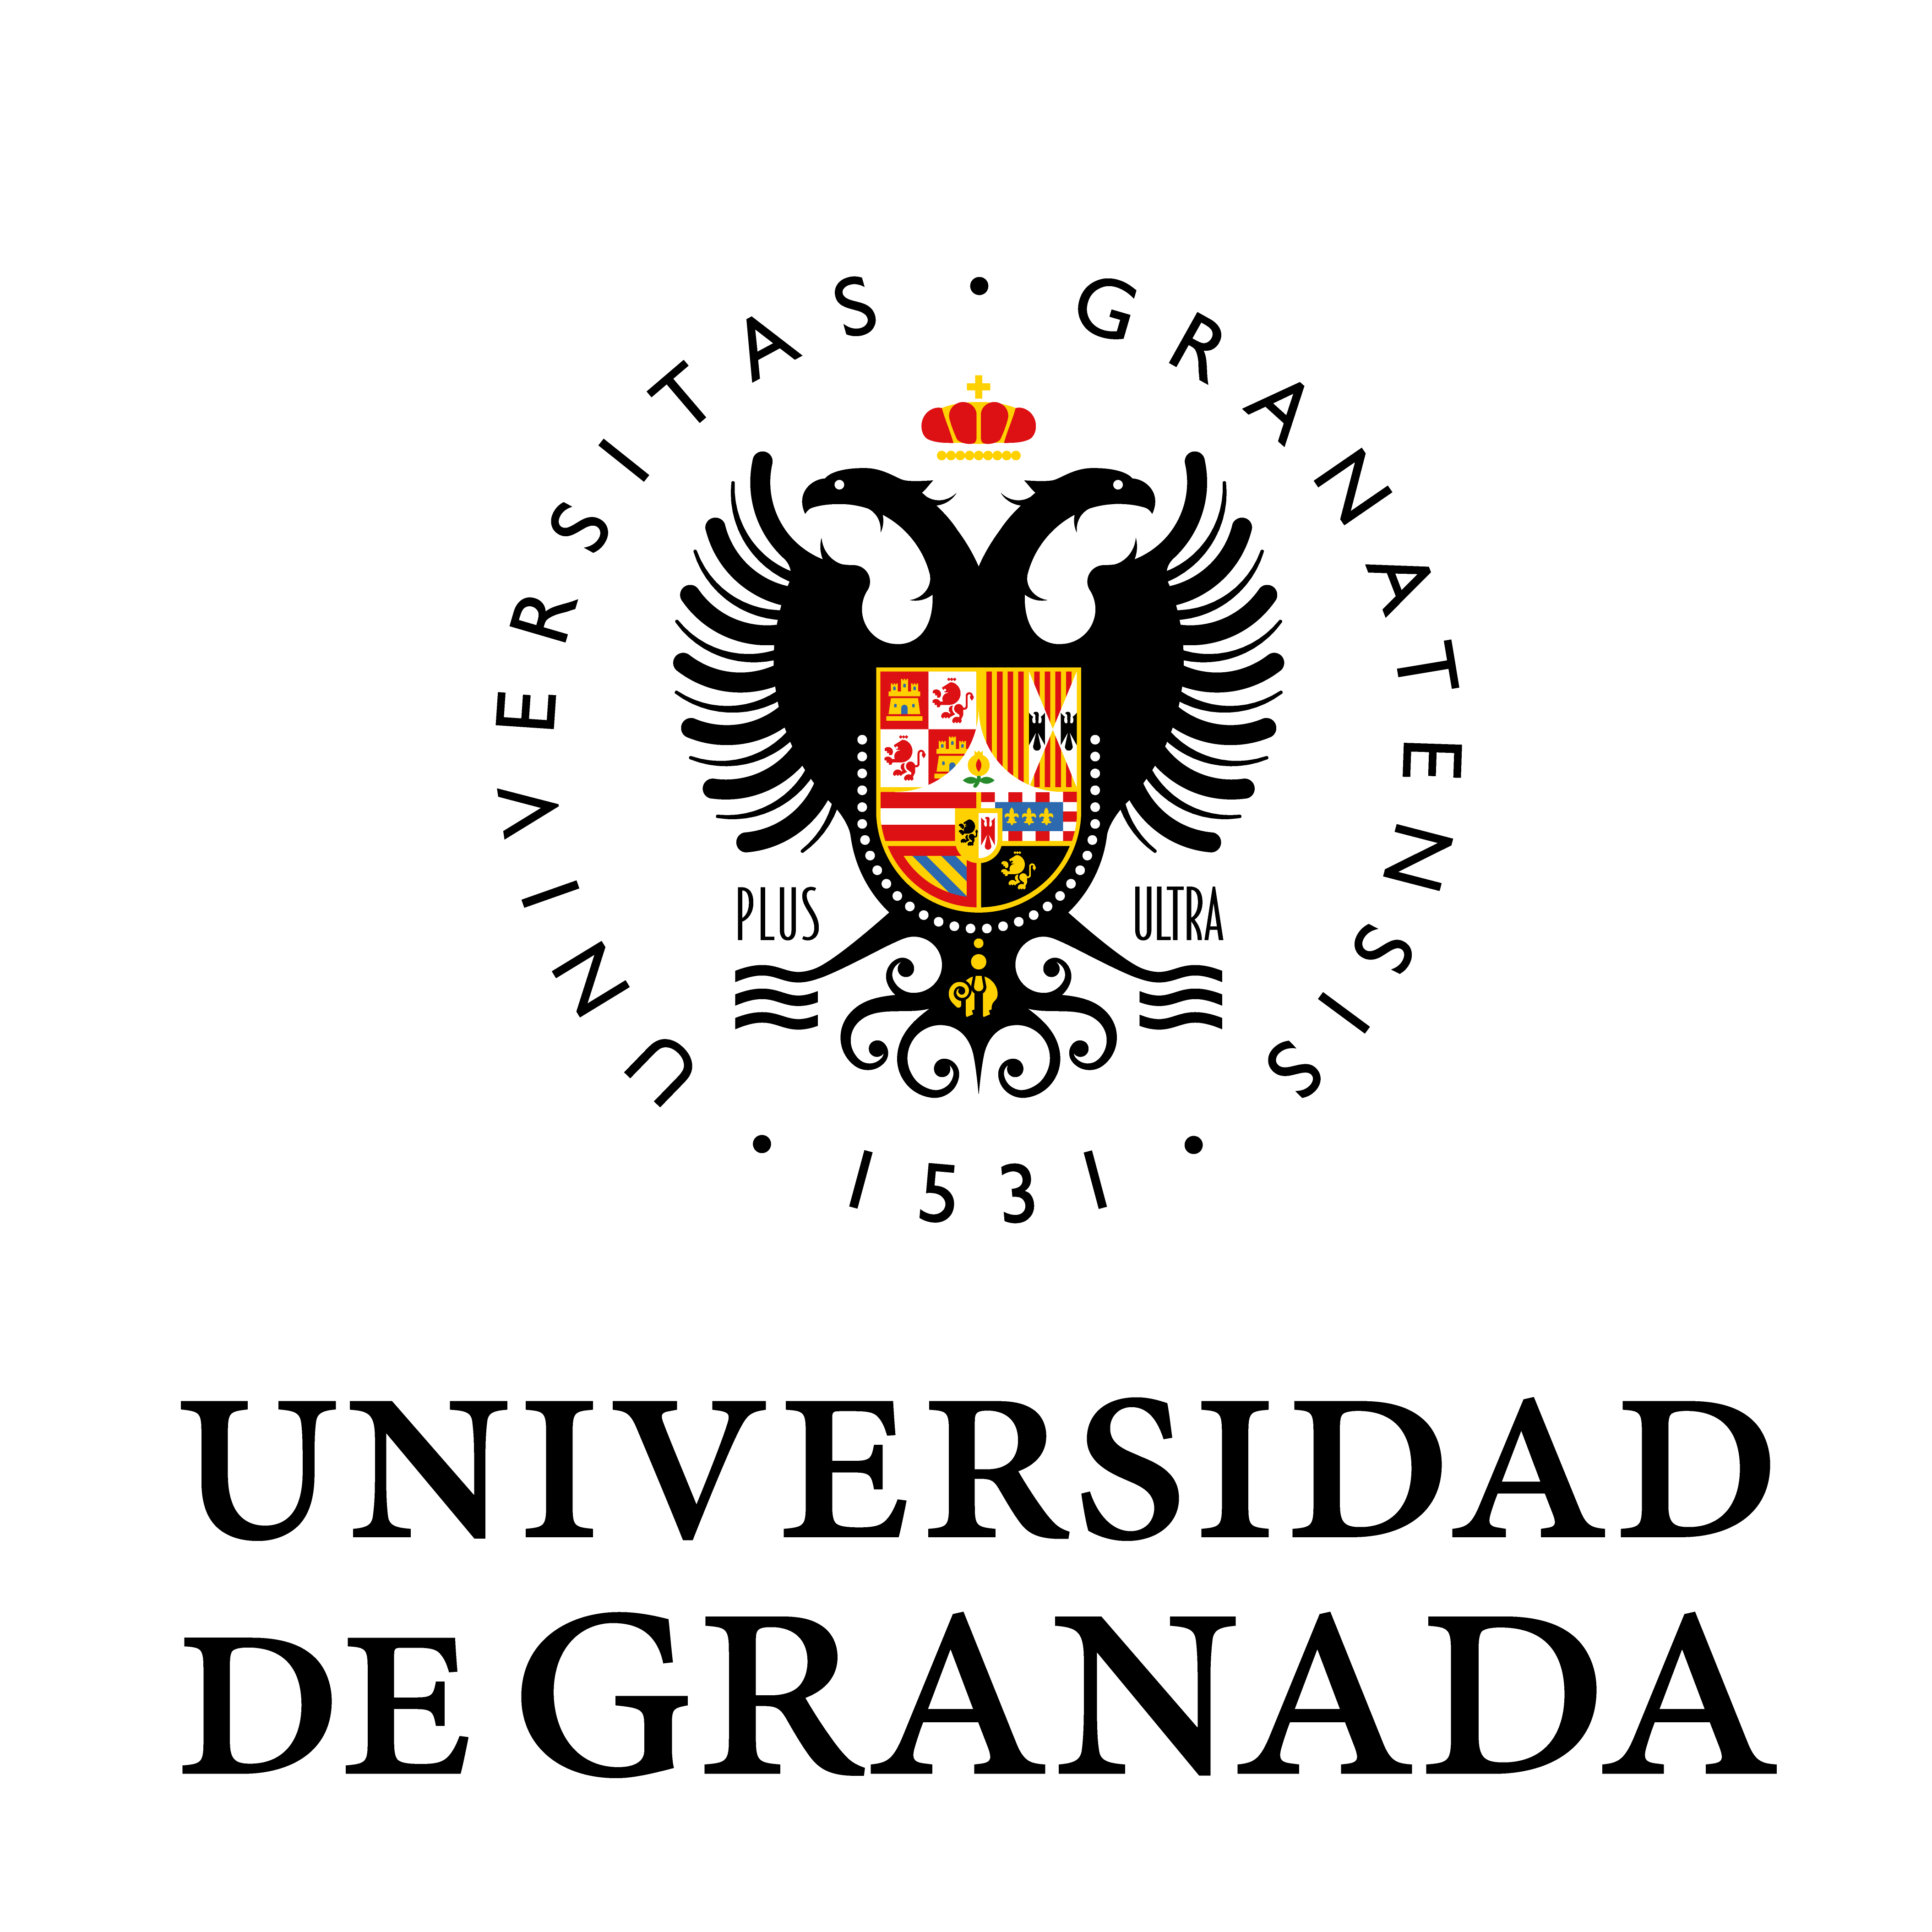
\includegraphics[width=0.5\textwidth]{images/logo-ugr.png}\par
    \vspace{1cm}
    {\Large\scshape Entornos Virtuales \par}
    {\huge\bfseries Interacción \par}
    \vspace{0.2cm}
    {\scshape Práctica 6 \par}
    \vfill
    {\large Víctor Vázquez Rodríguez  \par}
    {victorvazrod@correo.ugr.es \par}
    \vfill
    {\large Máster Universitario en Ingeniería Informática \par}
    \vspace{0.2cm}
    {Curso 2019/20 \par}
\end{titlepage}

En esta última práctica, el objetivo es permitir la interacción con la escena
que hemos diseñado. En mi caso, esta interacción consiste principalmente en
mover la locomotora, la cuál se comporta como avatar. Este movimiento se
implementa mediante sensores de teclado para las distintas teclas y actuadores
que se encargan de mover la locomotora. Los movimientos permitidos son los
siguientes:

\begin{itemize}
    \item \textbf{W} $\rightarrow$ Mover la locomotora en su eje Y (hacia
          adelante).
    \item \textbf{A y D} $\rightarrow$ Rotar la locomotora en torno a su eje Z a
          izquierda y derecha, respectivamente.
\end{itemize}

La lógica para estos movimientos se puede ver definida en la Figura
\ref{fig:locomotive} donde, además, se aprecia la otra interacción que se ha
añadido a la locomotora: la bocina. Al pulsar el botón izquierdo del ratón, la
locomotora produce un sonido de bocina de tren, el cuál se ha incorporado usando
un fichero MP3.

Como es de suponer, al mover la locomotora ésta tira del vagón, moviéndolo con
ella. No obstante, la bisagra que incorporamos en la práctica anterior para unir
estas dos piezas hace que se produzca una especie de efecto elástico al
producirse este movimiento, lo que hace difícil de controlar el vagón. Se ha
aumentado la masa de la locomotora para hacer que esto le afecte lo menos
posible.

\begin{figure}
    \centering
    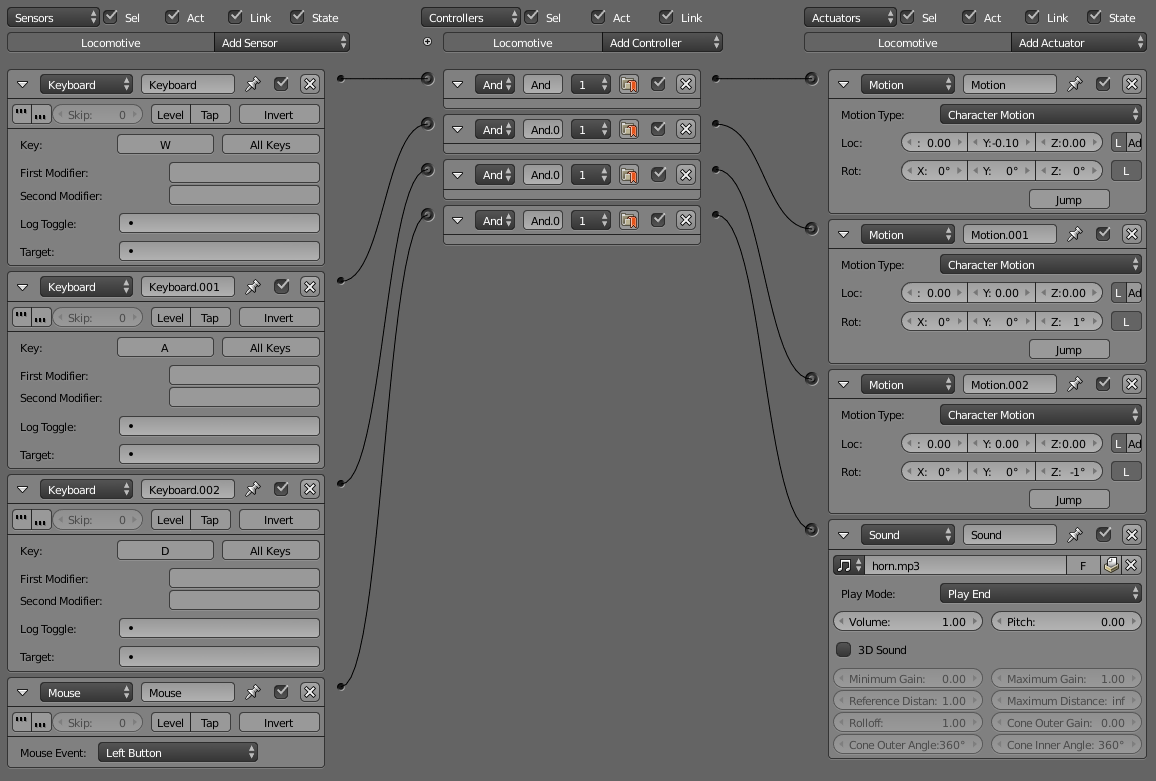
\includegraphics[width=\textwidth]{images/locomotive-logic.png}
    \caption{Lógica de movimiento de la locmotora y bocina}
    \label{fig:locomotive}
\end{figure}

La otra interacción que había que incorporar era la de la cámara, que debía
seguir siempre al avatar. En mi caso, he implementado este comportamiento de
forma diferente a la expuesta en el guión. Lo que he hecho ha sido incorporar
unos ejes vacíos a la jerarquía de la locomotora (\textit{Add} $\rightarrow$
\textit{Empty} $\rightarrow$ \textit{Plain Axes}) y establecer la cámara como
hija de estos ejes. Después, la lógica de movimiento de la cámara al mover el
ratón la definimos sobre los ejes en vez de sobre el objeto cámara. De esta
forma, conseguimos que la cámara siga al punto y esté siempre enfocándolo,
manteniendo la posición relativa al mismo que definimos en la escena. Esta
lógica de movimiento de la cámara se puede ver en la Figura \ref{fig:camera}, y
la posición de la misma, en la Figura \ref{fig:camera-position}.

\begin{figure}
    \centering
    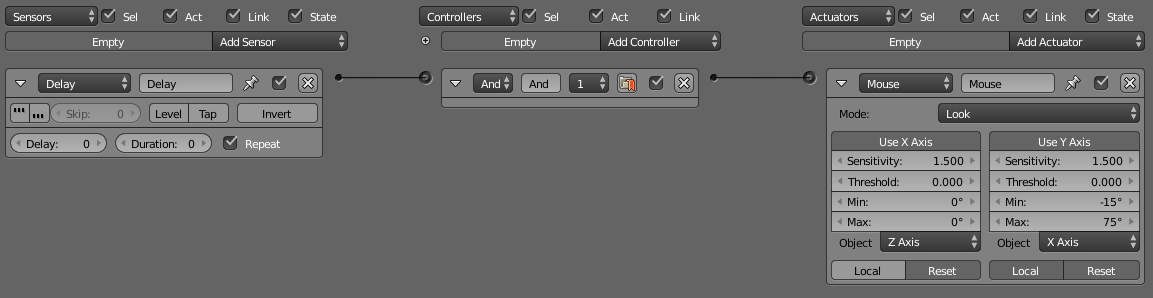
\includegraphics[width=\textwidth]{images/camera-logic.png}
    \caption{Lógica de movimiento de la cámara}
    \label{fig:camera}
\end{figure}

\begin{figure}
    \centering
    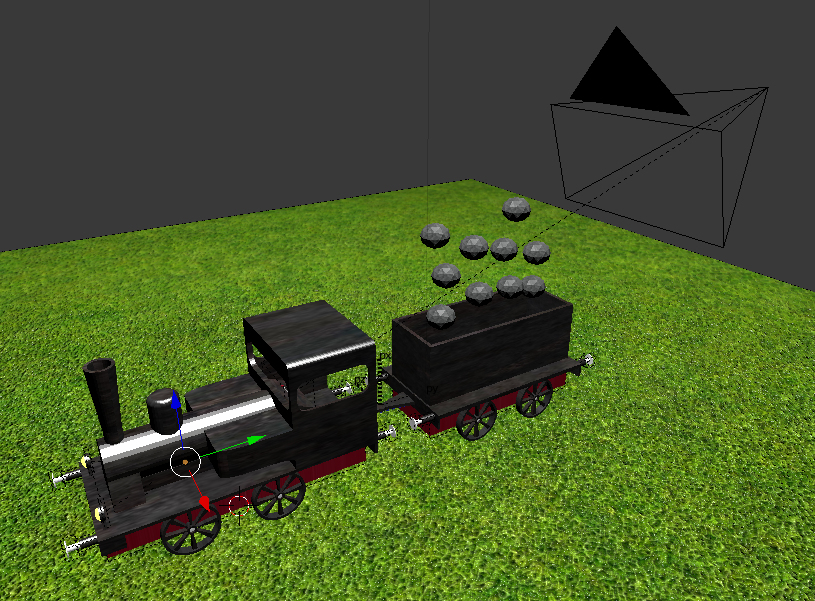
\includegraphics[width=\textwidth]{images/camera-position.png}
    \caption{Posición de la cámara respecto al centro de los ejes vacíos}
    \label{fig:camera-position}
\end{figure}

\end{document}
